%\subsection{Class Separability}



\section{Goodness Indicators}
\subsection{Classification With DTW and kNN}
\subsection*{Variable: $CO_2$ Concentration}
The first test is performed with $CO_2$ sensor from the bedroom 1 on the second floor (group 8 and sensor ID 646 in Table 2). The test data is from November 1st, 2012 until February 28th, 2013. One example week from that four month period is shown in Figure~\ref{fig:co2_1}. The classification levels defined in Chapter 4.1 are shown in the figure as well as one missing part that is covered with linear interpolation. For $CO_2$ the minimum level for an alert is set to S2, which is the red line in the picture.

\begin{center}
\begin{figure}[h!]
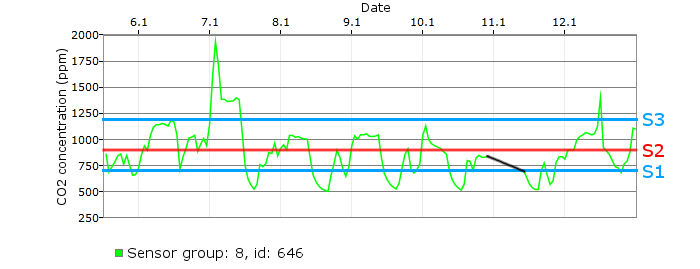
\includegraphics[scale=0.7]{images/co2_1.png}
\caption{Example time series from $CO_2$ sensor. The S1, S2 and S3 mark the classification limits.}
\label{fig:co2_1}
\end{figure}
\end{center}

First, let us investigate the effects of DTW and kNN parameters on the classification results. It is reasonable to suppose that the values of \emph{radius} and \emph{k} should have only a minor effect on the classification results. The time parameters were set to the following values
\begin{itemize}
\item{windowLength: 4 hours}
\item{windowDifference: 1 hour}
\item{waitingInterval: 30 min}
\item{eventInterval: 2 hours}
\item{exceedTime: 30 min}
\end{itemize}

These values mean that a new four-hour predictor vector is created every hour. This predictor is considered positive if the sensor value exceeds the limit value for 30 minutes within two hours after the predictor and a waiting time of 30 minutes.

A 30-day period from November 2012 with a total of 267,524 events was used to test the six parameter combinations. The first 70 \% of the data was used for training and the rest for testing. The classification results are shown in Table~\ref{table:co2_dtwknn_1}.


\begin{table}
  \caption{Results for November 2012 with DTW and kNN model ($W = 0.5$). The definition of ROC distance $AC_d$ is shown in (\ref{eq:acd}). For each row the number of positive samples is $\text{P} = \text{TP} + \text{FN} = 134$ and the number of negative samples is $\text{N} = \text{FP} = \text{TN} = 99$.} 
  \begin{tabular}{ c | c | c | c | c | c | c | c | c | c }
    \hline
   	\textbf{radius} & \textbf{k} & \textbf{TP} & \textbf{FP} & \textbf{TN} & \textbf{FN} & \textbf{TPR} & \textbf{FPR} & \textbf{Accuracy} & $\mathbf{AC_d}$ \\
	\hline
	5 & 3 & 110 & 18 & 81 & 24 & 0.92 & 0.13 & 0.82 & 0.16 \\
	5 & 7 & 103 & 8 & 91 & 31 & 0.77 & 0.060 & 0.83 & 0.17 \\
	5 & 15 & 101 & 9 & 90 & 33 & 0.75 & 0.067 & 0.82 & 0.18 \\
	50 & 3 & 108 & 15 & 84 & 26 & 0.81 & 0.11 & 0.82 & 0.16 \\
	50 & 7 & 102 & 7 & 92 & 32 & 0.76 & 0.052 & 0.83 & 0.17 \\
	50 & 15 & 103 & 6 & 93 & 31 & 0.77 & 0.045 & 0.84 & 0.17 \\
	\hline
  \end{tabular}
  \label{table:co2_dtwknn_1}
\end{table}

As can be seen from the results, the parameters \emph{radius} and \emph{k} do not have much effect on the classifier performance. Thus, the simplest possible model is selected. For the rest of the experiments values $radius = 5$ and $k = 3$ will be used.

Next, we perform the two experiments described in Chapter 4.4.2. The first test trains the model with 14 days of data and then runs tests in batches of 7 days. The second test runs three iterations, each beginning with a training period of 14 days and then three 7-day test batches. The parameters are the same as in the previous test except for the \emph{exceedTime} which is now set to 1 hour.

The results from these experiments are shown in Table~\ref{table:co2_dtwknn_2}. As can be seen from the table, there is no significant difference between constantly updating model and using the the same model for all tests.


\begin{table}
  \caption{DTW and kNN based model. 1: Periodically trained model. 2: Model that is trained only once.} 
  \begin{tabular}{ c | c | c | c | c }
    \hline
   	\textbf{Week} & \textbf{1: Purpose} & \textbf{1: Accuracy} & \textbf{2: Purpose} & \textbf{2: Accuracy} \\
	\hline
	1 & Training & - & Training & - \\
	2 & Training & - & Training & - \\
	3 & Testing & 0.72 & Testing & 0.72 \\
	4 & Testing & 0.81 & Testing & 0.81 \\
	5 & Testing & 0.71 & Testing & 0.71 \\
	6 & Training & - & Testing & 0.75 \\
	7 & Training & - & Testing & 0.86 \\
	8 & Testing & 0.88 & Testing & 0.94 \\
	9 & Testing & 0.91 & Testing & 0.94 \\
	10 & Testing & 0.75 & Testing & 0.75 \\
	11 & Training & - & Testing & 0.84 \\
	12 & Training & - & Testing & 0.86 \\
	13 & Testing & 0.76 & Testing & 0.72 \\
	14 & Testing & 0.81 & Testing & 0.83 \\
	15 & Testing & 0.81 & Testing & 0.84 \\
	\hline
  \end{tabular}
  \label{table:co2_dtwknn_2}
\end{table}

The $CO_2$ consumption seems to be quite easy to predict with this data set because the peaks are quite wide and they occur with constant intervals. The EPN is likely to capture two kinds of complex events: ones that actually precede peaks and ones that are within a peak indicating that the peak will continue.

As of the beginning of April, 2013, the test house was equipped with a mechanical ventilation system which improved the air quality significantly. This change eliminates the periodic increase in $CO_2$ levels we tried to predict in the previous tests. As a comparison, the model was evaluated with four one-week periods from March and April, 2013. These results are shown in Table~\ref{table:co2_dtwknn_3}.

\begin{table}
  \caption{Performance of DTW and kNN based model in the spring of 2013. The mechanical ventilation system was installed in the beginning of April.} 
  \begin{tabular}{ c | c | c | c | c | c | c | c | c | c | c }
    \hline
   	\textbf{Start} & \textbf{End} & \textbf{P} & \textbf{N} & \textbf{TP} & \textbf{FP} & \textbf{TN} & \textbf{FN} & \textbf{TPR} & \textbf{TNR} & \textbf{Accuracy} \\
	\hline
	01.03.13 & 08.03.13 & 42 & 61 & 19 & 1 & 60 & 23 & 0.45 & 0.98 & 0.77 \\
	08.03.13 & 15.03.13 & 17 & 70 & 7 & 1 & 69 & 10 & 0.41 & 0.99 & 0.87 \\
	15.03.13 & 22.03.13 & 11 & 76 & 2 & 2 & 74 & 9 & 0.18 & 0.97 & 0.87 \\
	29.03.13 & 06.04.13 & 32 & 57 & 25 & 0 & 57 & 7 & 0.78 & 1.00 & 0.92 \\
	06.04.13 & 13.04.13 & 2 & 83 & 0 & 3 & 80 & 2 & 0.00 & 0.96 & 0.94 \\
	13.04.13 & 20.04.13 & 2 & 83 & 0 & 2 & 81 & 2 & 0.00 & 0.98 & 0.95 \\
	20.04.13 & 27.04.13 & 2 & 83 & 1 & 1 & 82 & 1 & 0.50 & 0.99 & 0.98 \\
	\hline
  \end{tabular}
  \label{table:co2_dtwknn_3}
\end{table}

As can be seen from the number of positive testing samples in Table~\ref{table:co2_dtwknn_3}, the $CO_2$ levels decreased after the installation of mechanical ventilation system. Or at least the periodic peaks disappeared. The model now struggles with positive sample with \emph{TPR} being much worse than in the previous tests. In the winter the average \emph{TPR} was $0.76$ for the same model.


\subsection*{Variable: VOC}
As a second test variable we are using Volatile Organic Compounds (VOC). The sensor ID is 789 and the group is 7. It is located in a bedroom in the first floor. 

As the last chapter indicated, we would not get much advantage from parameter optimization. Thus, we continue using the same values $k = 3$ and $radius = 5$. A sample week of the data is shown in Figure~\ref{fig:voc_1}.

\begin{center}
\begin{figure}[h!]
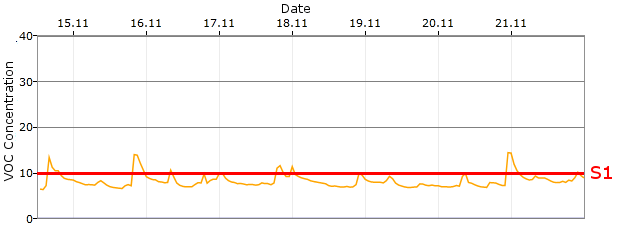
\includegraphics[scale=0.7]{images/voc_1.png}
\caption{VOC concentration.}
\label{fig:voc_1}
\end{figure}
\end{center}

As the figure shows, this time the peaks that exceed the limit value (S1) are much sharper. Thus, we first try to find the optimal time constants. The test data is again from November, 2012.

Two time parameters, \emph{windowDifference} and \emph{exceedTime}, are kept as constants with values 4 hours and 5 min respectively. A small \emph{exceedTime} is required to detect the sharp peaks. The prediction horizon parameters, \emph{windowLength}, \emph{waitingInterval} and \emph{eventInterval} are varied. For each combination a three-fold cross validation is performed and average performances are calculated. The results are shown in Table~\ref{table:voc_dtwknn_1}.

\begin{table}[here]
  \caption{Cross validation performances for DTW and kNN based model with different time parameters and VOC as measurand.} 
  \begin{tabular}{ c | c | c | c | c | c | c }
    \hline
   	\textbf{windowLength} & \textbf{waitingInterval} & \textbf{eventInterval} & \textbf{TPR} & \textbf{FPR} & \textbf{Accuracy} & $\mathbf{AC_d}$ \\
	\hline 
\rowcolor{Good}
2 hours & 30 min & 1  hour & 0.54 & 0.08 & 0.77 & 0.57 \\
\rowcolor{Good}
4 hours &  &  & 0.56 & 0.05 & 0.79 & 0.54 \\
8 hours &  &  & 0.38 & 0.09 & 0.71 & 0.68 \\
2 hours & 1  hour &  & 0.45 & 0.12 & 0.70 & 0.65 \\
\rowcolor{Good}
4 hours &  &  & 0.55 & 0.08 & 0.76 & 0.58 \\
8 hours &  &  & 0.34 & 0.14 & 0.64 & 0.71 \\
2 hours & 2 hours &  & 0.43 & 0.13 & 0.68 & 0.66 \\
4 hours &  &  & 0.48 & 0.07 & 0.73 & 0.62 \\
8 hours &  &  & 0.33 & 0.21 & 0.60 & 0.73 \\
2 hours & 30 min & 2 hours & 0.52 & 0.13 & 0.72 & 0.61 \\
\rowcolor{Good}
4 hours &  &  & 0.55 & 0.09 & 0.75 & 0.58 \\
8 hours &  &  & 0.38 & 0.18 & 0.63 & 0.70 \\
2 hours & 1  hour &  & 0.45 & 0.13 & 0.69 & 0.65 \\
\rowcolor{Good}
4 hours &  & & 0.57 & 0.08 & 0.77 & 0.57 \\
8 hours &  &  & 0.35 & 0.21 & 0.60 & 0.72 \\
2 hours & 2 hours &  & 0.43 & 0.13 & 0.67 & 0.66 \\
4 hours &  &  & 0.50 & 0.14 & 0.70 & 0.63 \\
8 hours &  &  & 0.34 & 0.22 & 0.59 & 0.73 \\
	\hline
  \end{tabular}
  \label{table:voc_dtwknn_1}
\end{table}

The results show that the model misclassifies too many positive samples as negatives. The best parameter combinations are highlighted in the table. Clearly \emph{windowLength} of 4 hours works best. Other two parameters do not show that clear impact so we choose 30 min for \emph{waitingInterval} and 1 hour for \emph{eventInterval} because they produce a simpler model.

The selected model is tested with data starting from the beginning of December 2012. Figure~\ref{fig:voc_dtwknn_test} shows True Positive Rate (\emph{TPR}) and False Positive Rate (\emph{FPR}) for each week.

\begin{center}
\begin{figure}[h!]
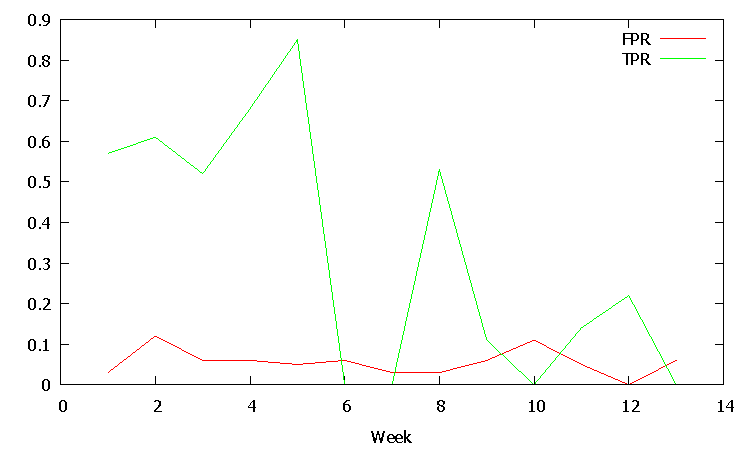
\includegraphics[scale=1.0]{images/voc_dtwknn_test.pdf}
\caption{Weekly \emph{TPR} and \emph{FPR} for DTW and kNN based model starting from the beginning of December 2012.}
\label{fig:voc_dtwknn_test}
\end{figure}
\end{center}

The \emph{FPR} is very small as it was in the parameter selection, too. The \emph{TPR} maintains its level at 0.50-0.60 for five weeks and then drops significantly. Looking at the data shows that the number of limit-exceeding peaks almost disappear in the wintertime. Thus, it is very difficult for the model to predict these rare events.

\subsection{Classification with Wavelets and SVMs}
\subsection*{Variable: CO2}
First, let us look at the product of the Haar Wavelet Transform. Figure~\ref{fig:wavelets} shows the original time series and Haar Wavelets with three different levels, 1, 2 and 10. The Weka Wavelet algorithm chooses the level from equation
\begin{align}
\mathbf{level} = \emph{ceil} \left ( \frac{\log{\emph{length}}}{\log{2}} \right ),
\end{align}
where \emph{length} is the length of the time series and \emph{ceil()} rounds the answer up to the nearest integer. When the length of the time series is about 1000 points, the equation gives 10 levels.


\begin{figure}[h!]
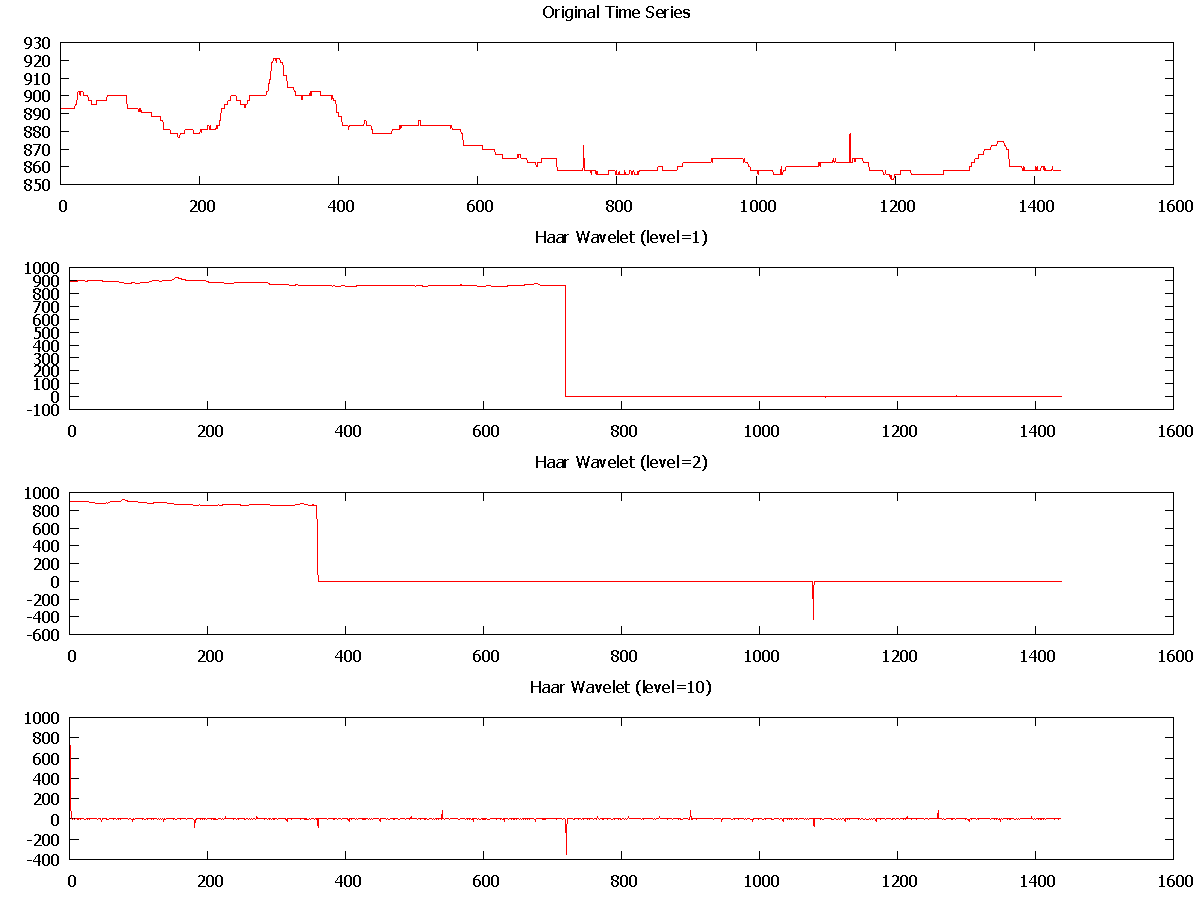
\includegraphics[scale=0.8]{images/wavelets.pdf}
\caption{Original time series and Haar Wavelets with three different levels, 1, 2 and 10.}
\label{fig:wavelets}
\end{figure}


This time the model parameters, $\gamma$ and \emph{C} should have a major impact on the classification results. Hence, we will perform an actual cross validation with 5 folds as described in Chapter 3.6.1. The data used is again from November 2012 so the resulting classifier can be compared to the one in the previous chapter.

For each parameter combination a cross validation is performed. Then, an average $AC_d$ from Equation~\ref{eq:acd} is calculated for each parameter combination. The best parameter combination is then used for training the model.

For parameter $\gamma$ the grid values are calculated using the Jaakkola Heuristics described in Equation~\ref{eq:svm_gamma} with $a_0$ set to five. This results in 11 different values for $\gamma$. For parameter \emph{C} we use a logarithmic grid $\{ 10^{i} \}$, $i = -2, ... 6$ to first find out the correct magnitude for \emph{C}.

The average accuracies and calculated $AC_d$s for \emph{C} and $\gamma$ are shown in Figures~\ref{fig:co2_svm_c} and \ref{fig:co2_svm_gamma}. Each point in the graphs is an average value of all the test runs with the given parameter value. There were a total of 55 runs for each value of \emph{C} and 45 runs for each value of $\gamma$.

\begin{center}
\begin{figure}[h!]
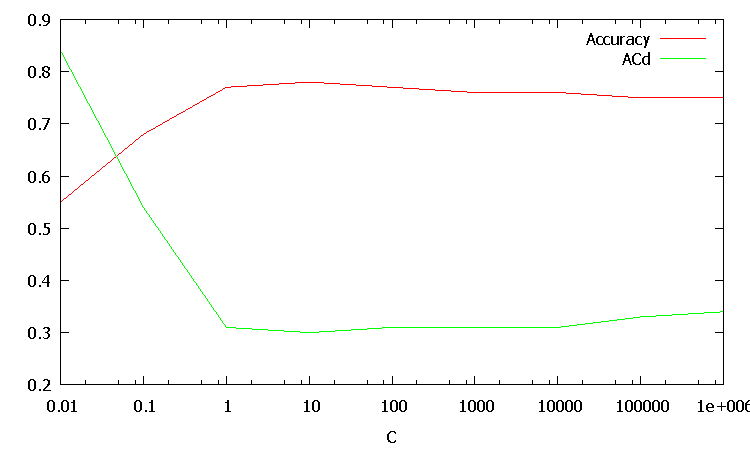
\includegraphics[scale=1.0]{images/co2_svm_c.pdf}
\caption{SVM classifier performance as a function of \emph{C}.}
\label{fig:co2_svm_c}
\end{figure}
\end{center}

\begin{center}
\begin{figure}[h!]
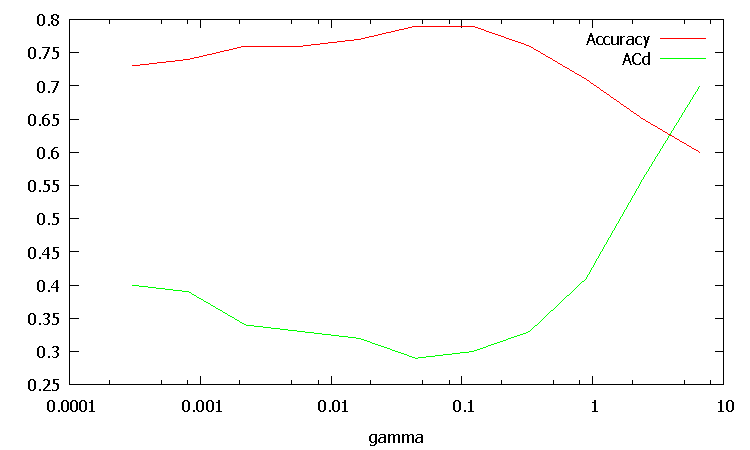
\includegraphics[scale=1.0]{images/co2_svm_gamma.pdf}
\caption{SVM classifier performance as a function of $\gamma$.}
\label{fig:co2_svm_gamma}
\end{figure}
\end{center}

The average classifier performance improves as \emph{C} increases to one. After that the accuracy decreases slowly. As the parameters might not be independent of each other, these graphs alone can not be used to select the optimal values. Figure~\ref{fig:co2_svm} shows accuracy as a function of both \emph{C} and $\gamma$. By inspecting the graphs a suitable combination for the parameters could be $C = 10$ and $\gamma = 0.05$. 

\begin{center}
\begin{figure}[h!]
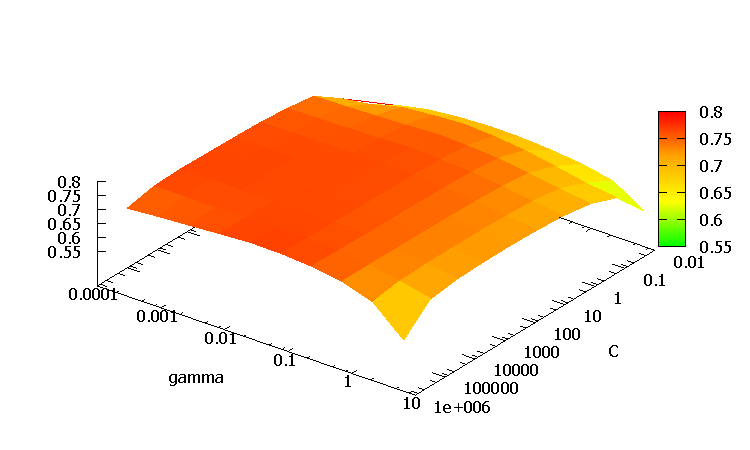
\includegraphics[scale=1.0]{images/co2_svm.pdf}
\caption{SVM classifier accuracy as a function of \emph{C} and $\gamma$.}
\label{fig:co2_svm}
\end{figure}
\end{center}

Next, the Wavelet and SVM model is trained with 14 days of data. This can not be done, however, with the same data we used for parameter selection because that approach would end up with overfitting. The values for \emph{TPR}, \emph{FPR} and Accuracy are shown in Figure~\ref{fig:co2_waveletsvm_test}.

The figure shows that the performance of this classifier varies much more than that of the DTW and kNN model.

\begin{center}
\begin{figure}[h!]
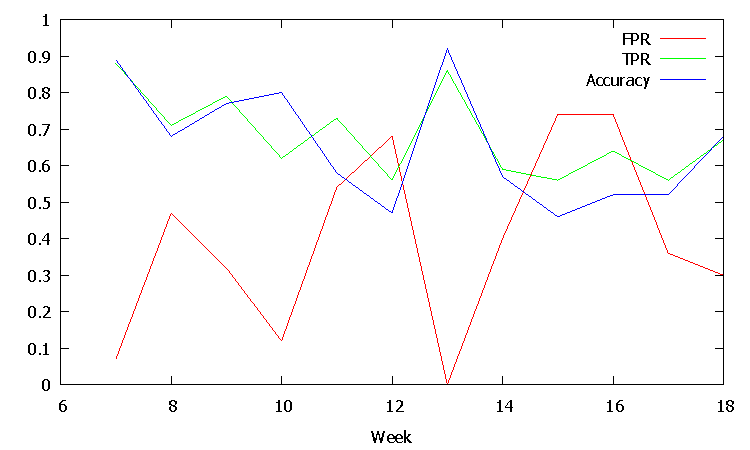
\includegraphics[scale=1.0]{images/co2_waveletsvm_test.pdf}
\caption{Wavelet and SVM based model performance with $C = 10$ and $\gamma = 0.05$.}
\label{fig:co2_waveletsvm_test}
\end{figure}
\end{center}



%\subsubsection*{Variable: VOC}
%We use the same data as for DTW and kNN based model in the %last section. Again, a grid search for optimal parameter %values is performed with data from November 2012. Since it %was shown with DTW and kNN model that the 

\section{Computational Performance}
Standard DTW algorithm has time complexity of $\mathcal{O}(N^2)$, where \emph{N} is the length of the time series. However, the FastDTW library we are using promises time complexity of $\mathcal{O} (N)$ \cite{salvador04}. The training phase of DTW and kNN is $\mathcal{O}(1)$ operation and takes only a few milliseconds because no calculations are performed. The given training set is simply saved into the model. Only when a new instance is classifier, DTW algorithm is run against each training sample and then \emph{k} closest are selected for voting.

\begin{center}
\begin{figure}[h!]
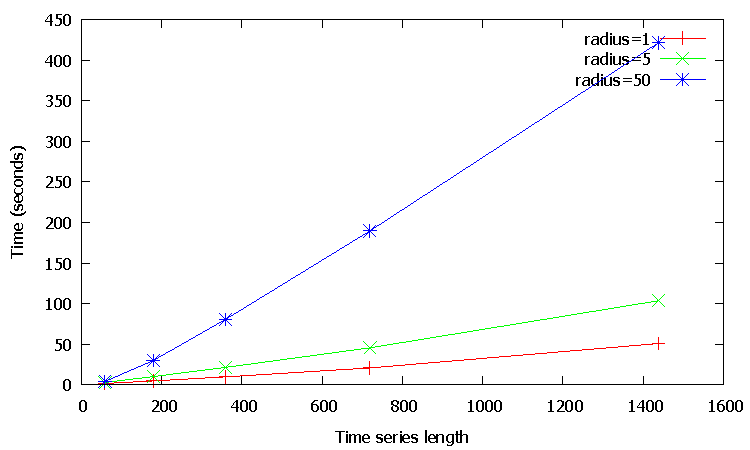
\includegraphics[scale=0.7]{images/dtw_knn_performance_timeseries_length.pdf}
\caption{DTW and kNN based model's performance as a function of time series length.}
\label{fig:dtw_knn_performance_timeseries_length}
\end{figure}
\end{center}

Figure~\ref{fig:dtw_knn_performance_timeseries_length} shows the training time as a function of time series length. Different time series lengths were acquired by varying the \emph{windowLength} parameter from 10 minutes to 4 hours. The smaller the \emph{radius} parameter is, the shorter the calculation time is as the algorithm is stopped earlier. As the authors of FastDTW promised, the time complexity is linear for relatively small time series ($< 2000$ data points). For longer time series it soon becomes second-degree polynomial. \cite{salvador04}




The LibSVM promises time complexity of $\mathcal{O}(l)$, where $l$ is the length of the time series if no kernel evaluations are required and $\mathcal{O}(nl)$ when $n$ kernel evaluations are required \cite{libsvm}. To put it briefly, the SVM training should be linear. 

\begin{center}
\begin{figure}[h!]
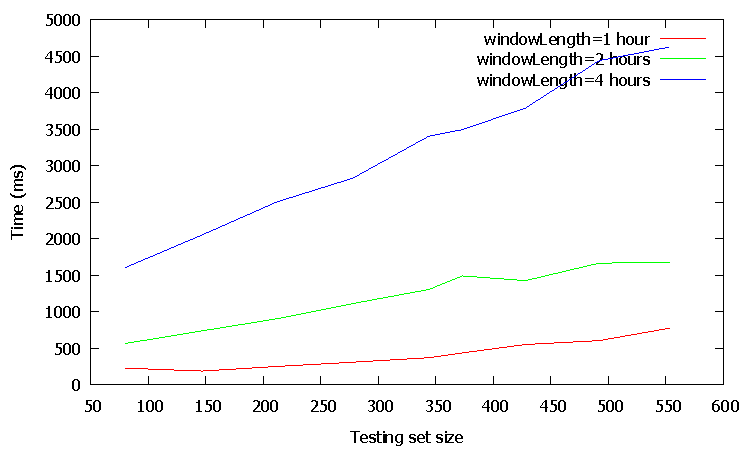
\includegraphics[scale=0.7]{images/wavelet_svm_performance.pdf}
\caption{Wavelet and SVM based model's performance as a function of training set size.}
\label{fig:wavelet_svm_performance}
\end{figure}
\end{center}

Figure~\ref{fig:wavelet_svm_performance} shows the testing time of Wavelet and SVM based model when the training set size is held constant at 139 data points. Clearly, increasing the number of test instances increases the execution time linearly. This same applies for DTW and kNN based model. 

If the number of test instances is also increased, the time complexity of DTW and kNN based model is no longer linear but rather follows a polynomial relationship, possibly a second-degree one. This is because each extra testing instance must be evaluated against each extra training set instance. The exact form of this polynomial could be found by regression analysis.

Wavelet and SVM based model, on the other hand, remains at linear computational time despite the increased number of both training and testing samples. This follows from the linear time requirements of both discrete Haar transform and  

\section{Discussion}
The biggest difference between the two models was the computational time needed to train and test the models. DTW and kNN based model takes about few minutes while with Wavelet and SVM based model only a few seconds are enough. 

Even though the FastDTW algorithm uses various methods, such as data abstraction and warping path constraints, to speed up the calculations, it still is a relatively slow algorithm. There is no way to decrease the number of DTW calculations as each testing instance must be evaluated against each training instance.

Calculating the Discrete Haar Wavelet Transform for small time series is not computationally demanding. It only consists of a series of addition and subtraction operations until the desired level is achieved. Weka Wavelet library doesn't provide any method to manually set to level up to which the transformation is performed. It would be useful to evaluate the classifier performance as a function level used for Haar Transform.

The core of LibSVM is written in C programming language which achieves better performance than if it was written in pure Java. LibSVM uses two techniques, shrinking and caching, to decrease the iteration time \cite{libsvm}. The shrinking method identifies and removes some bounded elements resulting in a smaller optimization problem. The quite advanced mathematics behind this method are not review here. The caching method stores kernel evaluations into memory for later use and thus avoids recalculations.

When it comes to classification performance, it was shown that regular peaks are much more predictable than ones that occur relatively rarely. With $CO_2$ the DTW and kNN based model achieved an acceptable performance with accuracy being over $80 \%$, True Positive Rate (TPR) over $75 \%$ and False Positive Rate (FPR) under $10 \%$. 

When comparing a model that was trained once to a model that was trained with regular intervals, no differences were found. The reason for these findings might be that the signal was close to a stationary process whose mean and variance remained about the same for the whole testing period. It was also shown that the installation of mechanical ventilation system changed the indoor air conditions dramatically and the performance of the classifier plummeted.

With VOC variable it was shown that the system's time parameters have a major impact on the performance. For example, the optimal choice of \emph{windowLength} parameter may increase the accuracy from about $60 \%$ to over $75 \%$. The number of indoor air particles decreased in the winter and the classifier failed heavily after that.


The Wavelet and SVM based model is difficult to tune. In addition to system's time parameters, it has two parameters, \emph{C} and $\gamma$ that derive from the mathematical equations. With $CO_2$ it was shown that both these parameters have optimal values that maximize the accuracy and minimize the $AC_d$. However, the testing accuracy varied a lot compared to the first model. LibSVM provides additional parameters, such as $\epsilon$ for stopping the iteration and weight parameters for different classes, that are sure to affect the observed performance but were not investigated here.

The second model is much more sensitive to the available data. Even small changes in the time parameters transformed the classifier from a nearly perfect one to a completely useless one. Especially with VOC, which has sharp peaks occurring rarely, this model lacks some kind of dynamic time parameter tuning that would optimize the length and the difference of the time windows on the go.

All in all, the results were quite close to my expectations. The easy-to-use DTW and kNN based model outperformed the more sophisticated Wavelet and SVM based model. The latter model, however, showed potential for predicting regular peaks in less time then the first model. With a little bit more parameter tuning I am pretty confident that Haar Wavelets and SVMs can work together with reasonable results.



